% !TeX program = pdflatex
\documentclass[11pt,a4paper]{article}

\usepackage[british]{babel}
\usepackage[T1]{fontenc}
\usepackage{amsmath,amssymb,mathtools}
\usepackage{amsthm}
\usepackage{bbm}
\usepackage{booktabs}
\usepackage{graphicx}
\usepackage{geometry}
\usepackage{microtype}
\usepackage{xcolor}
\usepackage{csquotes}
\usepackage{hyperref}
\usepackage[nameinlink,noabbrev]{cleveref}
\newcounter{sisection}
\renewcommand{\thesisection}{S\arabic{sisection}}
\crefname{sisection}{SI section}{SI sections}
\Crefname{sisection}{SI section}{SI sections}
\usepackage[utf8]{inputenc}


\geometry{margin=1in}

\hypersetup{
  colorlinks=true,
  linkcolor=blue!50!black,
  citecolor=blue!50!black,
  urlcolor=blue!50!black
}

% Vancouver-style: numbered citations in order of first appearance; square brackets via \cite / \parencite
\usepackage[style=numeric,backend=biber,sorting=none,giveninits=true,maxbibnames=99]{biblatex}
\addbibresource{references.bib}


\newcommand{\Var}{\operatorname{Var}}


\newcommand{\PEFrugbyMeanEta}{???}    \newcommand{\PEFrugbySdEta}{???}
\newcommand{\PEFrugbySuccess}{???}    \newcommand{\PEFrugbyNkpis}{???}
\newcommand{\PEFrugbyNgames}{???}     \newcommand{\PEFrugbyCIlo}{???}
\newcommand{\PEFrugbyCIhi}{???}
\newcommand{\PEFfootMeanEta}{???}     \newcommand{\PEFfootSdEta}{???}
\newcommand{\PEFfootSuccess}{???}     \newcommand{\PEFfootNkpis}{???}
\newcommand{\PEFfootNgames}{???}      \newcommand{\PEFfootCIlo}{???}
\newcommand{\PEFfootCIhi}{???}
\newcommand{\PEFtotalStudies}{???}
\newcommand{\PEFhealthMeanEta}{???}   \newcommand{\PEFhealthSdEta}{???}
\newcommand{\PEFhealthSuccess}{???}   \newcommand{\PEFhealthN}{???}
\newcommand{\PEFgenomicsMeanEta}{???} \newcommand{\PEFgenomicsSdEta}{???}
\newcommand{\PEFgenomicsSuccess}{???} \newcommand{\PEFgenomicsN}{???}
\newcommand{\PEFfinanceMeanEta}{???}  \newcommand{\PEFfinanceSdEta}{???}
\newcommand{\PEFfinanceSuccess}{???}  \newcommand{\PEFfinanceN}{???}
\newcommand{\PEFmfgMeanEta}{???}      \newcommand{\PEFmfgSdEta}{???}
\newcommand{\PEFmfgSuccess}{???}      \newcommand{\PEFmfgN}{???}
\newcommand{\PEFqOneMeanEta}{???}     \newcommand{\PEFqOneCIlo}{???}
\newcommand{\PEFqOneCIhi}{???}        \newcommand{\PEFqOneMLimpr}{???}
\newcommand{\PEFqTwoMeanEta}{???}     \newcommand{\PEFqTwoMLimpr}{???}
\newcommand{\PEFqThreeMeanEta}{???}   \newcommand{\PEFqThreeMLimpr}{???}
\newcommand{\PEFqFourMeanEta}{???}    \newcommand{\PEFqFourCIlo}{???}
\newcommand{\PEFqFourCIhi}{???}       \newcommand{\PEFqFourMLimpr}{???}
\newcommand{\PEFmlCorr}{???}          \newcommand{\PEFmlRsq}{???}
\newcommand{\PEFmlMAE}{???}           \newcommand{\PEFmlRMSE}{???}
% Pipeline output overrides the fallbacks above via \renewcommand:
\InputIfFileExists{scripts/paper_pipeline/outputs/numbers.tex}{}{}
\providecommand{\PEFmedianDeltaRatio}{???}
\InputIfFileExists{scripts/paper_pipeline/outputs/finalize_correlations.tex}{}{}
\newcommand{\Cov}{\operatorname{Cov}}
\DeclareMathOperator{\Corr}{Corr}
\newcommand{\ind}{\mathbbm{1}}

\title{Pairing Efficiency Does Not Decide Whether a Team KPI Should Be Relativised}

\author{%
  M.~R. Brown\textsuperscript{1,*},
  L.~P. Kilduff\textsuperscript{1},
  G.~A. Scott\textsuperscript{1},
  N. Dingle\textsuperscript{1},
  M. Evans\textsuperscript{2},
  D. O'Hara\textsuperscript{1}
  and
  D. Morris\textsuperscript{3}\\[0.6em]
  \normalsize
  \textsuperscript{1}Swansea University, Swansea, UK\\
  \textsuperscript{2}Scarlets, Llanelli, UK\\
  \textsuperscript{3}Swansea City AFC, Swansea, UK\\[0.4em]
  \textsuperscript{*}Corresponding author:
  \href{mailto:m.r.brown@swansea.ac.uk}{\texttt{m.r.brown@swansea.ac.uk}}%
}
\date{}

\begin{document}
\maketitle
\begin{abstract}
In rugby union and association football, a team key performance indicator can enter a match-outcome model as that team's own count or as the difference from the opponent. The Paired Efficiency Factor $\eta=(1+\kappa)/(1+\kappa-2\sqrt{\kappa}\,\rho)$ compares the variance of the difference with unpaired measurement of the same two counts. It generalises Fisher's paired efficiency to unequal variances. The four cells of $(\kappa,\rho)$ record whether pairing reduces variance and which side is more variable. They do not decide which feature to use.

Under the probit model, $I(X;Y)$ is a one-dimensional integral in the relative signal $d_{\mathrm{rel}}$. At a fixed ratio $\delta/\sigma_{\mathrm{A}}$, a larger $\eta$ raises $d_{\mathrm{rel}}$ and lowers $I(X;Y)$. Inside that model the relative feature is Bayes-sufficient, so the accuracy gain $\Delta\mathrm{ML}$ is at least zero, and the gain depends on $(d_{\mathrm{rel}},r_{AX})$, including a gain at the Fisher point $\eta=1$.

Across $\PEFtotalStudies$ rugby and football KPIs, $\eta$ does not line up with the accuracy change ($r=\PEFcorrEtaML$). Class separation $\hat d_Y$ does not either ($r=\PEFcorrIpredML$). Four pre-specified exemplars, one per cell at comparable class separation, have fold intervals that all cover zero. Healthcare, genomics, and finance show the same second-moment geometry and have no match outcome.

Pairing efficiency is a diagnostic of the difference. The predictive choice is a direct comparison, reported with an interval.
\end{abstract}

\section{Introduction}

\subsection{Absolute, relative, or paired features}

Match-outcome models in rugby union and association football often choose among three representations of a team key performance indicator (KPI): the home count $A$, the difference $D=A-B$ from the away count, or the pair $(A,B)$ \parencite{bennett2019descriptive,bennett2021predicting,mosey2020,scott2023urc,scott2023womens}.
Those studies usually compare absolute and relative columns by cross-validated accuracy under logistic regression \parencite{dixon1997,berrar2019}.
Relative formulations improve accuracy in the United Rugby Championship \parencite{scott2023urc}.
They show no improvement over absolute features in international women's rugby \parencite{scott2023womens} and in Australian sub-elite rugby \parencite{mosey2020}.
A six-league football preprint again finds that team--opponent differences outperform isolated team statistics \parencite{brito2026}.
None of those reports answers whether the KPIs are aligned with home win, how large the team-blocked gap of $D$ is relative to the pair, or whether pairing efficiency sorts that gap.

\subsection{Three questions}

This paper studies $\PEFrugbyNkpis$ United Rugby Championship KPIs and $\PEFfootNkpis$ English Championship KPIs over seasons 23/24--24/25.
Home is $A$ and away is $B$, so $D=A-B$.
The outcome is home win versus not.
The analysis is organised around three questions.

\begin{enumerate}
  \item Are these KPIs aligned with home win under the null $\beta_A+\beta_B=0$ in a logistic model of $(A,B)$?
  \item How large is the team-blocked out-of-sample log-loss gap of $D$ relative to $(A,B)$ and to $A$?
  \item Does the Paired Efficiency Factor $\eta$, or the quadrant of $(\kappa,\rho)$, sort that gap?
\end{enumerate}

Alignment means that the score from $(A,B)$ depends on the pair only through $D$.
The classical cost of a redundant coefficient is about $1/(2n_{\mathrm{train}})$ in expected test log-loss \parencite{akaike1973,stone1977}.
Both statements are recorded in Supplementary~\cref{sec:si_alignment}.
Because many KPIs may carry little signal beyond the home-win rate, the paper first reports leave-one-team-out skill against an intercept-only model and then answers the three questions for all KPIs and for an informative subset.

\subsection{Pairing efficiency is not the switch}

The variance of the difference is $\Var(A-B)=\sigma_A^2(1+\kappa-2\sqrt{\kappa}\,\rho)$ with $\kappa=\sigma_B^2/\sigma_A^2$ and $\rho=\Corr(A,B)$.
The Paired Efficiency Factor
\begin{equation}
  \eta = \frac{1+\kappa}{1+\kappa-2\sqrt{\kappa}\,\rho}
  \label{eq:pef}
\end{equation}
compares that variance with unpaired measurement of the same two counts \parencite{fisher1935}.
Paired-design theory suggests that differencing should help when pairing reduces variance.
Positive $\rho$ yields $\eta>1$; negative $\rho$ yields $\eta<1$.
The four cells of $(\kappa,\rho)$ record whether pairing reduces variance and which side is more variable.
They describe the KPI cloud.
They do not choose among $A$, $D$, and $(A,B)$.

\subsection{Scope and contributions}

\Cref{sec:theory} states $D$, the null, $\eta$, $r_A$, and the $1/(2n_{\mathrm{train}})$ cost.
\Cref{sec:methods} defines the likelihood-ratio statistic, leave-one-team-out log-loss, and the skill rule.
\Cref{sec:results} answers the three questions.
\Cref{sec:discussion} reads the medians against skill and the cost prediction.

The contributions are empirical.
First, intercept-only skill shows that most of these KPIs sit near the base rate, so alignment must not be over-read from null features.
Second, the sport-level distribution of $\Lambda$, with landmarks at $\PEFLRaic$ and $\PEFLRlandmark$.
Third, median team-blocked gaps that match $-1/(2n_{\mathrm{train}})$, with the finding that $\eta$ does not sort the $D$ versus $(A,B)$ gap.

\section{Theoretical Framework}
\label{sec:theory}

\subsection{Three feature sets}

Let $A$ be the home KPI and $B$ the away KPI on a match.
Write $D=A-B$.
A logistic model of home win may use one of three designs: the single feature $A$, the difference $D$, or the pair $(A,B)$.
Under the pair model the score is $\beta_0+\beta_A A+\beta_B B$.
Writing $S=A+B$, the linear score is $\tfrac12(\beta_A-\beta_B)D+\tfrac12(\beta_A+\beta_B)S$.
The null $\beta_A+\beta_B=0$ is therefore the restriction that the score depends on $(A,B)$ only through $D$.
When that restriction holds we call the KPI aligned.
The derivation is classical and is recorded in Supplementary~\cref{sec:si_alignment} \parencite{white1982}.

\subsection{Likelihood-ratio statistic}

On the full sample the likelihood-ratio statistic for $\beta_A+\beta_B=0$ is
\begin{equation}
  \Lambda = 2\bigl(\ell_{(A,B)}-\ell_D\bigr),
  \label{eq:lr}
\end{equation}
where $\ell$ is the maximised logistic log-likelihood.
Under independent observations the null reference is $\chi^2_1$ \parencite{wilks1938}.
Two landmarks are marked on the figure.
$\PEFLRaic$ is Akaike's one-parameter crossover for out-of-sample feature choice \parencite{akaike1973,stone1977}.
$\PEFLRlandmark$ is the upper $5\%$ point of $\chi^2_1$.
Neither mark is used as a per-KPI $p$-value.
Team recurrence makes matches dependent, so the $\chi^2_1$ reference is a landmark rather than a calibrated null.

\subsection{The Paired Efficiency Factor and \texorpdfstring{$r_A$}{rA}}

With $\kappa=\Var(B)/\Var(A)$ and $\rho=\Corr(A,B)$, the Paired Efficiency Factor is \cref{eq:pef}.
The formula is distribution-free given finite second moments.
It recovers Fisher's equal-variance gain $1/(1-\rho)$ when $\kappa=1$ \parencite{fisher1935}.
Positive $\rho$ yields $\eta>1$.
Negative $\rho$ yields $\eta<1$.
Paired-design theory suggests that differencing should help when pairing reduces variance.
This paper tests whether $\eta$ sorts the predictive gaps.
The algebraic correlation
\begin{equation}
  r_A=\Corr(A,D)=\frac{1-\rho\sqrt{\kappa}}{\sqrt{1+\kappa-2\sqrt{\kappa}\,\rho}}
  \label{eq:rA}
\end{equation}
is a different function of $(\kappa,\rho)$.
It is reported beside $\eta$ as a second candidate sorter of the $A$ versus $D$ gap.
The four cells of $(\kappa,\rho)$ record efficiency and which side is more variable.
They do not decide whether to use $A$, $D$, or $(A,B)$.

\subsection{Finite-sample cost}

When $D$ is aligned, fitting $(A,B)$ spends one redundant coefficient.
For a correctly specified regular model the leading excess test log-loss is $k/(2n)$ nats for a $k$-parameter fit \parencite{akaike1973,konishi2008}, so
\begin{equation}
  \mathbb{E}\bigl[\mathrm{LL}(D)-\mathrm{LL}(A,B)\bigr]\approx -\frac{1}{2n_{\mathrm{train}}}.
  \label{eq:halfn}
\end{equation}
The expansion does not require Gaussian features (Supplementary~\cref{sec:si_alignment}).
Under leave-one-team-out, $n_{\mathrm{train}}$ is the training-set size.
At the fold sizes of this study the median cost is $\PEFrugbyHalfN$ milli-nats in rugby and $\PEFfootHalfN$ milli-nats in football.
Further geometric identities appear in a companion manuscript \parencite{pefstatistics2026}.

\section{Methodology}
\label{sec:methods}

\subsection{Study Design}

The validation proceeds in three tiers. The first is an idealised probit simulation under (A1)--(A2) that evaluates the integral for $I(X;Y)$ (\cref{eq:mi_closed}) on a $(\kappa,\rho,\delta/\sigma_{\mathrm{A}})$ grid (Supplementary~\cref{sec:si_probit}). The second tier is the primary analysis of professional sports KPIs: the $\PEFtotalStudies{}$ rugby and football KPIs ($\PEFrugbyNkpis{}$ rugby, $\PEFfootNkpis{}$ football) on the $(\kappa,\rho)$ plane (\cref{fig:pef_landscape}; Supplementary~\cref{fig:si_ipred_vs_dml}), with four single-KPI exemplars chosen by the rule below (\cref{sec:exemplars,tab:exemplars}). The third tier is supporting validation in healthcare, clinical genomics, and finance. The objectives are to state $I(X;Y)$ under one generative model, describe what the four cells do and do not decide, and test whether the same $(\kappa,\rho)$ geometry appears outside sport.

\subsection{Primary Data: Sports KPIs}

The primary analysis uses match-level KPI data from two professional leagues:
\begin{itemize}
  \item \textbf{Rugby union.} United Rugby Championship ({URC}): $n=\PEFrugbyNgames$ games pooled across seasons 23/24 and 24/25 ($m=16$ teams; 18 regular-season rounds in which each team plays 12 opponents once and three opponents twice). KPIs include rucks won, kick metres, kicks from hand, carries, penalties conceded, turnovers won, and others (\cref{fig:pef_landscape}).
  \item \textbf{Football.} English Championship: $n=\PEFfootNgames$ games pooled across the same two seasons ($m=24$ teams, double round-robin). KPIs include duels, pressures, interceptions, fouls, and shot volume (\cref{fig:pef_landscape}). The outcome in both sports is a home win versus not: draws are coded as not a home win. The home-win rate is $\PEFrugbyHomeWinPct\%$ in rugby and $\PEFfootHomeWinPct\%$ in football, so a majority-class classifier is already accurate in rugby and only modestly above one half in football. Association-football score and outcome modelling has a long econometric lineage \parencite{dixon1997,boulier2003}, with contemporary machine-learning approaches incorporating domain knowledge \parencite{berrar2019}.
\end{itemize}
Head-to-head matchups provide natural pairing through shared environmental conditions (weather, venue, officiating), and KPI variability across matches is well documented in professional sport \parencite{malcata2014}. Those rugby union lines of work motivate treating head-to-head KPIs as a primary testbed for the present framework \parencite{bennett2019descriptive,bennett2021predicting,mosey2020,scott2023urc,scott2023womens}. The sports data are well suited to testing the framework because the KPIs span a range of correlation values (including negative correlation from competitive dynamics) and variance ratios, populating all four quadrants. To assess temporal stability, we compute $(\hat{\kappa},\hat{\rho})$ for each KPI in both seasons separately. \Cref{fig:pef_landscape} is the full cloud, by season. The four exemplars are \cref{tab:exemplars}.

\subsection{Supporting Data: Cross-Domain Validation}

To assess generalisability beyond sports, we applied the framework to three additional domains. Domain-level summaries are reported in \cref{tab:validation}; the supporting tier is summarised in \cref{tab:validation}, not as markers on the sports cloud.

\textbf{Healthcare.} Paired systolic ({BPXOSY1}) and diastolic ({BPXODI1}) blood pressure readings from the same oscillometric measurement event, drawn from the {NHANES} 2017 public-use examination file \texttt{P\_BPXO} \parencite{nhanes2017pbxo}. Each participant contributes one (systolic, diastolic) pair; pulse pressure $\mathrm{PP}=\mathrm{SBP}-\mathrm{DBP}$ is the relative feature, an established cardiovascular risk biomarker \parencite{franklin1999,blacher1999}. Observations with $\mathrm{SBP}\le\mathrm{DBP}$ were excluded as physiologically implausible ($N=10{,}352$ retained).

\textbf{Clinical Genomics.} Normalised {RNA}-seq gene-level expression from {GEO} series {GSE47462}: patient-matched normal breast tissue vs early neoplasia \parencite{geoGSE47462,brunner2014earlybreast}. Pairs were defined by shared subject identifiers in the series sample annotations. Genes were ranked by paired-differential signal before the PEF summary. That ranking preferentially retains genes with a large between-condition shift and, in a paired design, high $\rho$, so the share with $\hat\eta>1$ is not a random-gene rate.

\textbf{Finance.} Daily log returns for $\PEFfinanceN$ {S\&P}~100 constituents over the pinned window 2020--2023, obtained from Yahoo Finance, each paired with the {S\&P}~500 \parencite{sharpe1966,sharpe1994,fama1970,carhart1997,fama1993}. Label A is the index and label B is the constituent, so $\kappa=\mathrm{Var}(\mathrm{stock})/\mathrm{Var}(\mathrm{market})$. Stored $\kappa$ is above one for most names and the correlation is positive, which places the typical name in Quadrant~1. Swapping the labels would send $\kappa$ to $1/\kappa$ and move those names to Quadrant~2 without changing $\eta$.

\subsection{Parameter Estimation}

For each dataset, the variance ratio and correlation were estimated using standard sample estimators
\begin{equation}
  \hat{\kappa} = \frac{s^{2}_{\mathrm{B}}}{s^{2}_{\mathrm{A}}},
  \quad
  \hat{\rho} =
  \frac{\sum_{i=1}^{n}(X_{\mathrm{A},i}-\bar{X}_{\mathrm{A}})(X_{\mathrm{B},i}-\bar{X}_{\mathrm{B}})}
       {\sqrt{\sum_{i=1}^{n}(X_{\mathrm{A},i}-\bar{X}_{\mathrm{A}})^{2}
              \sum_{i=1}^{n}(X_{\mathrm{B},i}-\bar{X}_{\mathrm{B}})^{2}}}.
\end{equation}
Under bivariate normality (Assumption~(A1)), these are maximum likelihood estimators. PEF was computed by substituting into \cref{eq:pef}. For sports KPIs, index $i$ runs over fixtures; $X_{\mathrm{A},i}$ and $X_{\mathrm{B},i}$ denote the home and away KPI counts from game~$i$, so $(\hat\kappa,\hat\rho)$ characterise the cross-fixture distribution of those paired observations rather than correlation within a single match or serial correlation of one team's time series.

\subsection{Empirical Units and Outcome Definitions}
\label{sec:outcome_defs}

Each sports KPI is one PEF unit: match-level home and away measurements pooled across seasons 23/24 and 24/25, yielding a single $(\hat\kappa,\hat\rho,\hat\eta)$ estimate per KPI. There are $\PEFtotalStudies{}$ such units ($\PEFrugbyNkpis{}$ rugby union, $\PEFfootNkpis{}$ football). Score, scoring events, cards, expected-goals and on-ball-value models, and shots on target are omitted, because those quantities are circular with the binary match outcome. Action KPIs (passes, carries, shot volume, tackles) are retained. Per-KPI estimates and season-to-season positions are in \cref{fig:pef_landscape}. Class separation against $\Delta\mathrm{ML}$, and the quadrant table, are in Supplementary~\cref{sec:si_landscape} (\cref{fig:si_ipred_vs_dml}).

Two reporting roles are distinguished. \textbf{Descriptive mapping} uses all rugby and football KPIs to show where they sit on the $(\kappa,\rho)$ plane, to summarise domain-level distributions, and to place them on \cref{fig:pef_landscape}. These aggregates are descriptive: $\PEFlandscapeQthreePct\%$ of the KPIs lie in Quadrant~3, so pooled statistics primarily reflect the dominant negative-correlation regime rather than a balanced sample of the quadrant space. \textbf{Illustrative checks} use four exemplars, one per quadrant (\cref{tab:exemplars}). The estimate of whether $\hat\eta$ tracks $\Delta\mathrm{ML}$ is the full cloud (Supplementary~\cref{fig:si_ipred_vs_dml}), together with the probit grid as a model check (Supplementary~\cref{sec:si_probit}). The exemplar rule is fixed before looking at $\Delta\mathrm{ML}$. Within a quadrant, keep KPIs with $|\log\hat\kappa|>\log 1.05$, so $\hat\kappa$ lies outside $[1/1.05,\,1.05]$ and the pick is not on the $\kappa=1$ boundary. Among those, choose the KPI whose absolute class separation $|\hat d_Y|$ is closest to the median $|\hat d_Y|$ of that eligible set. Walk Quadrants~1 to~4 and skip a name that contains, or is contained in, a name already chosen, so two versions of the same construct are not both used. If a quadrant has no eligible KPI the margin is relaxed to $\log 1.02$ and then to zero, and the margin actually used is recorded. Class separation is \cref{eq:class_sep}, with $Y$ the home-win indicator. The home--away gap $(\bar X_{\mathrm{A}}-\bar X_{\mathrm{B}})/s_{\mathrm{A}}$ is kept in the per-KPI export as a description of the two teams. It is not plugged into $I(X;Y)$. The four selected KPIs have $\hat d_Y$ from $\PEFexDeltaRatioLo$ to $\PEFexDeltaRatioHi$. Supplementary~\cref{tab:si_quad_landscape} summarises the remaining rugby and football KPIs by quadrant.

Where domain summaries report the proportion of KPIs with $\hat\eta>1$, this is the share for which pairing reduces variance relative to independent measurement. That share is a descriptive summary of the $(\kappa,\rho)$ distribution, not a hypothesis-test outcome; quadrant-level aggregates appear in Supplementary~\cref{tab:si_quad_landscape}.

\subsection{Machine Learning Validation}
\label{sec:ml_cv}

To assess the relationship between quadrant position and ML performance, logistic regression was fitted with five-fold cross-validation \parencite{kohavi1995}, implemented in {MATLAB} (\texttt{glmfit}, Statistics and Machine Learning Toolbox). The signed change $\Delta\mathrm{ML}=100(\mathrm{acc}_{\mathrm{rel}}-\mathrm{acc}_{\mathrm{abs}})/\mathrm{acc}_{\mathrm{abs}}$ compares the relative feature $X_{\mathrm{A}}-X_{\mathrm{B}}$ with the absolute feature $X_{\mathrm{A}}$. For the exemplars we also fit the two-feature logistic on $(X_{\mathrm{A}},X_{\mathrm{B}})$, and we report AUC, Brier score, and the majority-class accuracy. The point estimate in \cref{tab:exemplars} is the mean of the five fold-wise changes, with a paired $t$ interval on four degrees of freedom. That interval is a description of fold-to-fold variation. It is not a cluster-robust confidence interval for a super-population of leagues. Positive $\Delta\mathrm{ML}$ means the relative feature classified more accurately in these folds. Negative $\Delta\mathrm{ML}$ means it classified less accurately. The home--away gap is not used as the signal in this comparison. Class separation is \cref{eq:class_sep}.

\textbf{Team-blocked cross-validation.} Each match is one observation, but teams recur across fixtures, so random match-level folds can place the same side in both training and test sets and inflate accuracy. We partition home teams (not matches) into five disjoint sets with a fixed random seed. A match is assigned to the fold of its home team. For fold~$f$, the test set is the matches whose home team belongs to set~$f$, and the training set is the remaining matches. No home team therefore appears in both partitions within a fold. Away matches of a held-out club can remain in training when that club is the away side, so the block is not a full club hold-out. The same fold assignment is used for the absolute feature, the relative feature, and the two-feature model. Pooled $\Delta\mathrm{ML}$ values describe the rugby and football KPIs. Claims about sign use the fold intervals on the full set, including the Quadrant~3 counts in \cref{sec:exemplars}. The four exemplars illustrate the rule at typical $|\hat d_Y|$.

\subsection{Inference and Quality Control}
\label{sec:qc}

The $\PEFtotalStudies{}$-KPI landscape is descriptive. It is not a family-wise hypothesis battery, so Bonferroni, FDR, and Holm corrections are not applied. Uncertainty for $(\hat\kappa,\hat\rho,\hat\eta)$ uses a team-cluster bootstrap: teams are resampled with replacement and all home-side matches for each drawn team are retained ($B=1{,}000$) \parencite{efron1979}. That bootstrap, like the cross-validation, holds out home-team blocks, so away matches of the same club can remain in the resample. Supplementary~\cref{sec:si_qc} reports the check. Predictive comparisons use team-blocked $\Delta\mathrm{ML}$ (\cref{sec:ml_cv}).

Paired-difference series were checked with the Shapiro--Wilk test on the two-season window. The difference series rejects normality for $\PEFrugbySwReject\%$ of rugby KPIs and $\PEFfootSwReject\%$ of football KPIs (Supplementary~\cref{sec:si_normality}). Mean $W$ remains high ($0.977$ in rugby and $0.986$ in football). Several KPIs are low-count discrete series, so a rejection can reflect that discreteness. The PEF formula uses second moments and does not require the rejection rate to be zero. Analysis code was version-controlled. The canonical run is \texttt{run\_paper\_pipeline.m} in {MATLAB} {R2025b} with the Statistics and Machine Learning Toolbox (\cref{sec:data_availability}).

\subsection{Sports Data: Independence Considerations}

The sports datasets present a hierarchical structure requiring careful treatment. Each team appears in multiple games, inducing correlation across observations involving the same team through latent team ability $\theta_{j}$:
\begin{equation}
  X_{j,i} = \theta_{j} + \epsilon_{j,i}.
\end{equation}
We model game-level observations using a bivariate normal approximation
\begin{equation}
  \bigl(X_{\mathrm{A}(i)}, X_{\mathrm{B}(i)}\bigr) \sim \mathcal{N}(\boldsymbol{\mu},\boldsymbol{\Sigma}),
  \quad i=1,\ldots,n,
\end{equation}
treating games as conditionally independent. Three considerations justify this approximation for PEF analysis:
\begin{enumerate}
  \item \textbf{Target of inference.} PEF focuses on cross-fixture (same-occasion) correlation $\rho=\Corr(X_{\mathrm{A},i},X_{\mathrm{B},i})$ summarised over fixtures $i=1,\ldots,n$, capturing shared environmental factors and competitive dynamics on each game occasion rather than serial dependence of a single team across games. Team quality primarily affects mean structure rather than the correlation structure driving PEF.
  \item \textbf{Variance estimation.} The total variance $\sigma^{2}_{\mathrm{A}}=\Var(\theta_{j})+\Var(\epsilon_{j,i})$ correctly reflects the observable variance relevant to feature engineering decisions.
  \item \textbf{Robustness checks.} For $(\hat\kappa,\hat\rho,\hat\eta)$, bootstrap confidence intervals resample \emph{teams} with replacement and retain all home-side matches for each drawn team (cluster bootstrap on the home-team index; Supplementary~\cref{sec:si_qc}). For predictive validation, team-blocked cross-validation (\cref{sec:ml_cv}) prevents home teams from appearing in both training and test folds. Together, these checks address the main dependence induced by recurring teams without altering the distribution-free PEF formula itself.
\end{enumerate}
This parallels established practice in sports analytics \parencite{benaim2006,owen2014} and panel data econometrics \parencite{cameron2015,wooldridge2010}.

\section{Results}
\label{sec:results}

\subsection{Skill and the base rate}
\label{sec:skill}

An intercept-only leave-one-team-out model has median log-loss $\PEFrugbyMedLLint$ nats in rugby and $\PEFfootMedLLint$ nats in football, close to the home-win-rate entropies ($0.643$ and $0.688$ nats at the rates in \cref{sec:methods}).
Median skill across KPIs is $\PEFrugbyMedSkill$ milli-nats in rugby and $\PEFfootMedSkill$ milli-nats in football.
Only $\PEFrugbyNinfo$ of $\PEFrugbyNkpis$ rugby KPIs and $\PEFfootNinfo$ of $\PEFfootNkpis$ football KPIs meet the informative rule (skill bootstrap interval excludes zero).
For the median KPI, $A$, $D$, and $(A,B)$ therefore sit near the base rate.
Alignment and gap comparisons below are reported for all KPIs and, where sample size allows, for the informative subset.

\subsection{Alignment with home win}
\label{sec:alignment}

\Cref{fig:e6_alignment}~(A) shows the distribution of $\Lambda$ for $\beta_A+\beta_B=0$.
In rugby the median is $\PEFrugbyMedLR$ (quartiles $\PEFrugbyLRqI$, $\PEFrugbyLRqIII$).
In football the median is $\PEFfootMedLR$ (quartiles $\PEFfootLRqI$, $\PEFfootLRqIII$).
Solid and dashed lines mark $\PEFLRaic$ (Akaike / CV crossover) and $\PEFLRlandmark$ ($\chi^2_1$ $5\%$ point).
Most KPIs sit below $\PEFLRaic$: $\PEFrugbyNaboveTwo$ rugby and $\PEFfootNaboveTwo$ football KPIs exceed $2$, and $\PEFrugbyNaboveChi$ and $\PEFfootNaboveChi$ exceed $3.84$.
The sport-level quartiles sit modestly to the right of the $\chi^2_1$ null quartiles ($0.10$, $0.45$, $1.32$), but KPIs are correlated within a match, so the $86$ statistics are not independent draws.
No per-KPI $p$-value is claimed.

\subsection{Team-blocked log-loss gaps}
\label{sec:gaps}

\Cref{fig:e6_alignment}~(B) shows per-KPI gaps $\mathrm{LL}(D)-\mathrm{LL}(A,B)$ in milli-nats.
Dashed segments mark $-1/(2n_{\mathrm{train}})$ at the sport median fold size ($\PEFrugbyHalfN$ milli-nats in rugby; $\PEFfootHalfN$ in football).
Across all KPIs the median gap is $\PEFrugbyMedGapDf$ milli-nats in rugby ($[\PEFrugbyMedGapDfLo,\PEFrugbyMedGapDfHi]$) and $\PEFfootMedGapDf$ in football ($[\PEFfootMedGapDfLo,\PEFfootMedGapDfHi]$).
Both intervals contain the corresponding $-1/(2n_{\mathrm{train}})$ prediction.
The median $A$ versus $D$ gap is $\PEFrugbyMedGapAD$ milli-nats in rugby and $\PEFfootMedGapAD$ in football.
On the informative subset the median $D$ versus $(A,B)$ gap is $\PEFrugbyMedGapDfInfo$ milli-nats in rugby ($n=\PEFrugbyNinfo$) and $\PEFfootMedGapDfInfo$ in football ($n=\PEFfootNinfo$).
With so few informative KPIs those subset medians are descriptive only.

\subsection{Do \texorpdfstring{$\eta$}{eta} or \texorpdfstring{$r_A$}{rA} sort the gap?}
\label{sec:eta_sort}

Within sport, the correlation of $\hat\eta$ with the $D$ versus $(A,B)$ gap is $\PEFrugbyCorrEtaDf$ in rugby and $\PEFfootCorrEtaDf$ in football.
The correlation of $\hat\eta$ with the $A$ versus $D$ gap is $\PEFrugbyCorrEtaAD$ and $\PEFfootCorrEtaAD$.
The correlation of $\hat r_A$ with the $A$ versus $D$ gap is $\PEFrugbyCorrRAAD$ and $\PEFfootCorrRAAD$.
Neither $\eta$ nor the quadrant sorts the $D$ versus $(A,B)$ gap.
The $r_A$ association with the $A$ versus $D$ gap has the expected sign (smaller $r_A$, larger advantage of $D$ over $A$) but is modest in football.
On the informative subset the same pattern appears with very small $n$ ($\PEFrugbyCorrRAADInfo$ rugby; $\PEFfootCorrRAADInfo$ football).
The KPI cloud occupies all four cells and concentrates in Quadrant~3 (\cref{fig:pef_landscape}): rugby $\PEFrugbyQone$/$\PEFrugbyQtwo$/$\PEFrugbyQthree$/$\PEFrugbyQfour$ and football $\PEFfootQone$/$\PEFfootQtwo$/$\PEFfootQthree$/$\PEFfootQfour$ across Q1--Q4.
That count describes the landscape.
It does not choose the feature.

\subsection{Pre-specified exemplars}
\label{sec:exemplars}

\Cref{tab:exemplars} reports the four pre-specified KPIs with bootstrap intervals.
None is informative under the skill rule.
The table illustrates one cell per quadrant.
It is not an estimate of the sport-level median.

\begin{table}[ht]
  \centering
  \caption{Pre-specified exemplars (one KPI per quadrant).
    Gaps are team-blocked log-loss differences in milli-nats, with bootstrap intervals.
    Skill is likewise in milli-nats.
    Informative means the skill interval excludes zero.}
  \label{tab:exemplars}
  \scriptsize
  \setlength{\tabcolsep}{3pt}
  \begin{tabular}{@{}llccccccc@{}}
    \toprule
    Sport & KPI & $\hat\eta$ & $\hat r_A$ & $\Lambda$ & Skill & $\mathrm{gap}(D,(A,B))$ & $\mathrm{gap}(A,D)$ & Info \\
    \midrule
    \PEFexQoneSport & \PEFexQoneKPI & \PEFexQoneEta & \PEFexQoneRA & \PEFexQoneLR & \PEFexQoneSkill &
      $\PEFexQoneGapDf$ $[\PEFexQoneGapDfLo,\PEFexQoneGapDfHi]$ &
      $\PEFexQoneGapAD$ $[\PEFexQoneGapADLo,\PEFexQoneGapADHi]$ & \PEFexQoneInfo \\
    \PEFexQtwoSport & \PEFexQtwoKPI & \PEFexQtwoEta & \PEFexQtwoRA & \PEFexQtwoLR & \PEFexQtwoSkill &
      $\PEFexQtwoGapDf$ $[\PEFexQtwoGapDfLo,\PEFexQtwoGapDfHi]$ &
      $\PEFexQtwoGapAD$ $[\PEFexQtwoGapADLo,\PEFexQtwoGapADHi]$ & \PEFexQtwoInfo \\
    \PEFexQthreeSport & \PEFexQthreeKPI & \PEFexQthreeEta & \PEFexQthreeRA & \PEFexQthreeLR & \PEFexQthreeSkill &
      $\PEFexQthreeGapDf$ $[\PEFexQthreeGapDfLo,\PEFexQthreeGapDfHi]$ &
      $\PEFexQthreeGapAD$ $[\PEFexQthreeGapADLo,\PEFexQthreeGapADHi]$ & \PEFexQthreeInfo \\
    \PEFexQfourSport & \PEFexQfourKPI & \PEFexQfourEta & \PEFexQfourRA & \PEFexQfourLR & \PEFexQfourSkill &
      $\PEFexQfourGapDf$ $[\PEFexQfourGapDfLo,\PEFexQfourGapDfHi]$ &
      $\PEFexQfourGapAD$ $[\PEFexQfourGapADLo,\PEFexQfourGapADHi]$ & \PEFexQfourInfo \\
    \bottomrule
  \end{tabular}
\end{table}

\section{Discussion}
\label{sec:discussion}

\subsection{Why Relativisation Helps and Harms}

Relativisation helps or harms according to a KPI's $(\kappa,\rho)$ regime. At matched signal the exemplars confirm both signs (\cref{tab:exemplars}). The studies that motivated this work framed the choice as help versus no help \parencite{bennett2019descriptive,bennett2021predicting,mosey2020,scott2023urc,scott2023womens}. They did not classify a regime in which the difference is the worse classifier. The Quadrant~3 result is that missing regime.

Quadrant membership remains a coarse guide. The PEF surface is nonlinear in $(\kappa,\rho)$ and $\delta/\sigma_{\mathrm{A}}$, so two KPIs in the same quadrant need not share the same $\Delta\mathrm{ML}$. The confirmatory table tests local agreement with the taxonomy, not a linear quadrant effect.

The analysis is univariate by design. Those same motivating studies used multi-KPI classifiers, where inter-feature correlations and joint decision boundaries lie outside univariate PEF. Reported $\Delta\mathrm{ML}$ values here are therefore conservative: they benchmark one paired feature at a time (\cref{sec:ml_cv}), and the exemplars test directional agreement rather than match-outcome accuracy.

\subsection{Efficiency versus Information}

Statistical efficiency ($\eta$) and predictive power ($I(X;Y)$) are functionally related through \cref{eq:mi_closed}, yet they measure different things. Classical variance-reduction reasoning advises against relativisation when $\eta<1$. That rule addresses only one dimension of the feature choice. It does not account for information content.

The PEF formula (\cref{eq:pef}) requires only finite second moments. The information-content relationship requires bivariate normality (A1). The efficiency characterisation is therefore the more general result. Relative gain when $\eta<1$ is a property of information content, not a failure of $\eta$.

\subsection{Practical Guidance}
\label{sec:practical_guidance}

The first two answers yield a prior for the feature choice:
\begin{enumerate}
  \item Estimate $\kappa$ and $\rho$ from available data.
  \item Compute $\eta$ using \cref{eq:pef}.
  \item Identify the quadrant from \cref{tab:quadrants}.
  \item For Quadrants~1--2, use relative features (they improve both statistical efficiency and information content).
  \item For Quadrant~3, prefer absolute features: relativisation is predictively harmful.
  \item For Quadrant~4, estimate $\delta/\sigma_{\mathrm{A}}$ from the same sample and confirm the sign of $\Delta\mathrm{ML}$ under team-blocked cross-validation. The (A1)--(A2) formula for $I(X;Y)$ is a prior for whether relativisation could help, not a substitute for that check.
\end{enumerate}
Possession-normalised rates are a different construction from opponent differences \parencite{sever2026}. They adjust for game state rather than pairing two teams' counts. The signed-harm recommendation in step~5 applies to opponent pairing, not to that rate construction. An open implementation is provided (Supplementary~\cref{sec:si_practitioner}; \cref{sec:data_availability}).

\subsection{The Same Geometry Outside Sport}

The third question is whether the same geometry appears outside sport. Market-adjusted returns, paired clinical designs, control charts, and relative sports metrics are instances of correlation-based variance reduction with different $(\kappa,\rho)$ values. A further analogue is value-added benchmarking in education, which compares teacher performance with that of comparable cohorts \parencite{hanushek2010}.

Healthcare pairing sits in Quadrant~2 (\cref{tab:validation}), the high-$\rho$ regime in which the taxonomy recommends relative features. Invasion-game KPIs occupy all four quadrants and concentrate in Quadrant~3 (\cref{sec:results}). Relativisation helps for some sports measurements and is harmful for others because $(\kappa,\rho)$ differs by KPI, not because sport is a single regime.

\subsection{Limitations}

\textbf{Distributional assumptions.} The PEF formula is distribution-free, but the information content relationship (\cref{eq:mi_closed}) assumes bivariate normality. Paired differences are often closer to normal than the raw series (Supplementary~\cref{sec:si_normality}). Strongly skewed or multimodal distributions may still need a non-parametric mapping. For count-based KPIs, $Z=\log(X+1)$ can improve normality whilst preserving the $(\kappa,\rho)$ structure. Across \PEFrugbyNkpis{} rugby KPIs the rank ordering by $\rho$ was largely preserved (Spearman $r_{s}=0.967$), and the aggregate PEF change was not significant ($\bar{\eta}_{\log}/\bar{\eta}=1.085$, $p=0.357$; Supplementary~\cref{sec:si_qc}). Individual count-based KPIs can still move substantially (rucks won).

\textbf{Stationarity.} The framework treats $\kappa$ and $\rho$ as fixed. Among the rugby and football KPIs, most drift modestly between seasons 23/24 and 24/25, though a minority of rugby KPIs cross quadrant boundaries (\cref{fig:pef_landscape,fig:info_surface}; Supplementary~\cref{fig:si_kpi_labelled}). Pooled two-season estimates (as in \cref{tab:exemplars}) therefore summarise a moving target.

\textbf{Binary outcomes.} Both \cref{eq:mi_closed} and the sports protocol target binary classification: which team wins a head-to-head match. That choice matches the probit link under (A1)--(A2) and keeps the KPI comparison on a common scale. Multi-class outcomes and continuous targets would need a corresponding information-theoretic mapping. The per-KPI $(\kappa,\rho)$ diagnostic still applies wherever paired absolute and relative features can be formed.

\textbf{Strategic interactions.} In invasion-game sport, teams respond to opponents' tactics and game state. The $(\kappa,\rho)$ structure of a KPI is therefore partly an equilibrium property of competition, not a fixed physical law. Parameters here are estimated from observed match data without a model of within-game adaptation. Where such dynamics are material, $(\kappa,\rho)$ should be read as descriptive summaries at the chosen time scale.

\textbf{Primary evidence base.} The rugby and football KPIs, the machine-learning validation, and the quadrant exemplars are the primary evidence. Healthcare, clinical genomics, finance, and manufacturing show that the same $(\kappa,\rho)$ geometry recurs (\cref{tab:validation}), but without the same per-unit ML scrutiny or temporal replication.

\subsection{Future Directions}

A priority is a distribution-free analogue of $I(X;Y)$, for example a rank-based or permutation measure. Quadrant~4 decisions would then not rely on (A1)--(A2) when skewness or heavy tails are material (Supplementary~\cref{sec:si_qc}).

Multivariate PEF-style summaries would show how per-KPI effects combine when several paired features enter one classifier. A complementary test is within-quadrant sampling: stratify high and low $\kappa$ and high and low $|\rho|$ inside each quadrant, with $\delta/\sigma_{\mathrm{A}}$ held comparable. That design would ask whether $\Delta\mathrm{ML}$ tracks local iso-$\eta$ or iso-$I(X;Y)$ structure rather than quadrant labels alone.

Rolling-window or state-space estimates of $(\kappa,\rho)$ would track parameter drift. Season-blocked or chronological cross-validation would tighten temporal leakage beyond the team-blocked folds used here (\cref{sec:ml_cv}).

Relativisation is often justified as baseline cancellation rather than variance reduction. Connecting PEF geometry to causal estimands would show when differencing preserves a treatment or exposure contrast and when it introduces collider or selection bias.

Deeper per-unit machine-learning checks in social-science panels, environmental paired measurements, and engineering telemetry would test whether the taxonomy transfers before the practical guidance is used outside invasion-game sport.

\section{Conclusion}

The paper asked three questions about the absolute-versus-relative choice.
Why does relativisation help for some KPIs and harm others?
How can a relative feature with $\eta<1$ still inform?
Does the same pairing geometry appear beyond sport?

Help and harm follow from two properties of each paired KPI: the variance ratio $\kappa=\sigma^{2}_{\mathrm{B}}/\sigma^{2}_{\mathrm{A}}$ and the within-match correlation $\rho$.
The Paired Efficiency Factor $\eta=(1+\kappa)/(1+\kappa-2\sqrt{\kappa}\,\rho)$ compares the variance of the difference with unpaired measurement.
The formula is distribution-free and contains Fisher's equal-variance result as the case $\kappa=1$.
Positive $\rho$ reduces that variance ($\eta>1$); negative $\rho$ inflates it ($\eta<1$).
That is why some KPIs should be relativised on efficiency grounds and others should not.
Efficiency is not the same as information about the outcome.
Under bivariate normality, $\eta$ and $I(X;Y)$ are related through the signal strength $\delta/\sigma_{\mathrm{A}}$, the standardised mean difference between the two entities.
A relative feature can therefore improve prediction when $\eta<1$, provided the mean separation remains large relative to the amplified noise.

For the rugby and football KPIs, $\kappa$ is the variance ratio of the two teams.
The correlation $\rho$ measures whether their values rise and fall together or against each other.
Those coordinates place every KPI in one of four quadrants.
Rugby and football occupy all four and concentrate in Quadrant~3, where $\kappa<1$ and $\rho<0$, so absolute features are preferred.
Four exemplars at comparable $\delta/\sigma_{\mathrm{A}}$ confirm both help and harm (\cref{tab:exemplars}).
The same $(\kappa,\rho)$ geometry appears in healthcare, clinical genomics, finance, and manufacturing, with different mean $\hat\eta$ (\cref{tab:validation}).
Quadrant membership is a first-pass guide for the feature choice.
Signal strength $\delta/\sigma_{\mathrm{A}}$ then scales how much of that geometry appears in prediction.
In Quadrant~4 it is required before a relative feature is retained.

\section{Data and Code Availability}
\label{sec:data_availability}

Rugby union KPIs were supplied by Oval Insights through access arranged with Scarlets RFC and are not redistributed.
Football KPIs were analysed under agreement with Swansea City AFC and are not redistributed.

Team-blocked log-loss, skill, and likelihood-ratio statistics were produced by \path{Alternative Pipeline/pef_numerics/experiments/E6_sports.py}.
Second-moment landscape files were produced by \path{scripts/paper_pipeline/run_paper_pipeline.m} in {MATLAB} {R2025b} with the Statistics and Machine Learning Toolbox.
Macros in \path{scripts/paper_pipeline/outputs/sports_numbers.tex} are regenerated from those CSVs without refitting.
A de-identified per-KPI table, with no match rows, is written to \path{scripts/paper_pipeline/outputs/referee_kpi_summary.csv}.
Analysis code will be deposited with the accepted manuscript; match-level KPI files remain under the data agreements above.

\section{Author Statements}
\label{sec:author_statements}

The blanks below are for the authors to complete before submission.

\subsection{CRediT}

M.~R. Brown: conceptualisation, methodology, software, formal analysis, writing (original draft). [Co-author name]: [contribution].

\subsection{Funding}

[Funder and grant number, or a statement that the work received no specific grant.]

\subsection{Competing interests}

Rugby KPIs were supplied through access arranged with Scarlets RFC (affiliation of M.~Evans).
Football KPIs were analysed under agreement with Swansea City AFC (affiliation of D.~Morris).
[Other relationships to declare, or a statement that the authors have none.]

\subsection{Ethics}

The sports KPIs are secondary operational records used for this analysis. [Ethics committee name and reference, or the secondary-use decision the authors will cite.]

% Consolidated tables matching the manuscript numbering (Tables 1--2, 5).
% Tables 3--4 appear in \texttt{results.tex} with the subsections that discuss them.

\begin{table}[p]
  \centering
  \caption{Validation results across domains.}
  \label{tab:validation}
  \small
  \scalebox{0.9}{
  \begin{tabular}{@{}llccccl@{}}
    \toprule
    \textbf{Domain} & \textbf{Tier} & \textbf{$n$ units} & \textbf{Mean $\eta$} & \textbf{SD} & \textbf{\% with $\eta>1$} & \textbf{Data source} \\
    \midrule
    Sports (Rugby)      & Primary    & \PEFrugbyNkpis  & \PEFrugbyMeanEta  & \PEFrugbySdEta  & \PEFrugbySuccess\%  & {URC} \\
    Sports (Football)   & Primary    & \PEFfootNkpis   & \PEFfootMeanEta   & \PEFfootSdEta   & \PEFfootSuccess\%   & English Championship \\
    Healthcare          & Supporting & $\PEFhealthN^{\dagger}$ & \PEFhealthMeanEta & $\PEFhealthSE^{\dagger}$ & \PEFhealthSuccess\% & \cite{nhanes2017pbxo} \\
    Clinical Genomics   & Supporting & $\PEFgenomicsN^{\ddagger}$ & \PEFgenomicsMeanEta & \PEFgenomicsSdEta & \PEFgenomicsSuccess\% & \cite{brunner2014earlybreast,geoGSE47462} \\
    Finance             & Supporting & \PEFfinanceN    & \PEFfinanceMeanEta & \PEFfinanceSdEta & \PEFfinanceSuccess\% & Yahoo Finance \\
    \bottomrule
  \end{tabular}}
  \normalsize

  \medskip
  \begin{minipage}{0.95\linewidth}\small
    \textit{Note:} Proportion with $\hat\eta>1$: share of units for which pairing reduces variance (\cref{sec:outcome_defs}). The $n$ units column counts PEF units, not participants: healthcare is one paired study of $N=10{,}352$ participants. $^{\dagger}$Paired {NHANES} oscillometric records (systolic vs diastolic, first reading); the SD column is the bootstrap standard error $\PEFhealthSE$ for the pooled $\eta$. $^{\ddagger}$Genes in the ranked subset of the {GSE47462} paired design (see Methods). That ranking prefers high $\rho$, so the percentage with $\eta>1$ is not a random-gene rate. Primary empirical tier: the sports cloud in \cref{fig:pef_landscape} and class separation against $\Delta\mathrm{ML}$ in Supplementary~\cref{fig:si_ipred_vs_dml}; the four exemplars are \cref{tab:exemplars}. Supporting tier: parameter estimation and PEF calculation summarised here and in \cref{sec:results}.
  \end{minipage}
\end{table}

\begin{table}[p]
  \centering
  \caption{Quadrant taxonomy and practical guidance.}
  \label{tab:quadrants}
  \begin{tabular}{@{}lllll@{}}
    \toprule
    \textbf{Q} & \textbf{Parameters} & $\eta$ & \textbf{What the cell records} & \textbf{Feature choice} \\
    \midrule
    Q1 & $\kappa>1$, $\rho>0$  & $>1$  & Efficient; B more variable & Not settled by the cell \\
    Q2 & $\kappa<1$, $\rho>0$  & $>1$  & Efficient; A more variable & Not settled by the cell \\
    Q3 & $\kappa<1$, $\rho<0$  & $<1$  & Inefficient; A more variable & Not settled by the cell \\
    Q4 & $\kappa>1$, $\rho<0$  & $<1$  & Inefficient; B more variable & Not settled by the cell \\
    \bottomrule
  \end{tabular}

  \medskip
  \begin{minipage}{0.95\linewidth}\small
    $\eta>1$ if and only if $\rho>0$. The $\kappa=1$ split swaps if A and B are swapped. $I(X;Y)$ is not ranked by quadrant (\cref{eq:mi_closed}). Under (A1)--(A2), $\Delta\mathrm{ML}\ge 0$. On the sports KPIs the cell does not decide the feature: the fold intervals do not separate the sign (\cref{sec:exemplars}).
    \textbf{Examples:} Q1, market-adjusted returns with A the index; Q2, the {NHANES} systolic--diastolic pair; Q3, high-volume anti-correlated sports KPIs; Q4, sports KPIs with the away side more variable and $\rho<0$.
  \end{minipage}
\end{table}

\begin{table}[p]
  \centering
  \caption{Boundary behaviour (illustrative).}
  \label{tab:boundary}
  \begin{tabular}{@{}lccc@{}}
    \toprule
    \textbf{Condition} & $\eta$ & $I(X;Y)$ & \textbf{Interpretation} \\
    \midrule
    $\kappa=1$, $\rho=0$ (Fisher) & 1.000 & 0.252 & Balanced variances, no correlation \\
    $\kappa\to 0$                 & 1.000 & 0.227 & Entity B negligible; $d_{\mathrm{rel}}\to 1$ \\
    $\kappa\to\infty$             & 1.000 & 0.279 & $d_{\mathrm{rel}}\to 0$; outcome nearest balance \\
    $\rho\to -1$ ($\kappa=1$)     & 0.500 & 0.265 & Maximum variance amplification \\
    $\rho\to +1$ ($\kappa=1$)     & $\to\infty$ & $\to 0$ & $d_{\mathrm{rel}}\to\infty$; outcome nearly certain \\
    \bottomrule
  \end{tabular}

  \medskip
  \begin{minipage}{0.95\linewidth}\small
    \textit{Note:} $I(X;Y)$ is \cref{eq:mi_closed} at $\delta/\sigma_{\mathrm{A}}=1$. As $d_{\mathrm{rel}}$ grows, $H(Y)$ falls, so the $\rho\to +1$ limit is $0$ bits rather than $1$ bit.
  \end{minipage}
\end{table}

\begin{figure}[p]
  \centering
  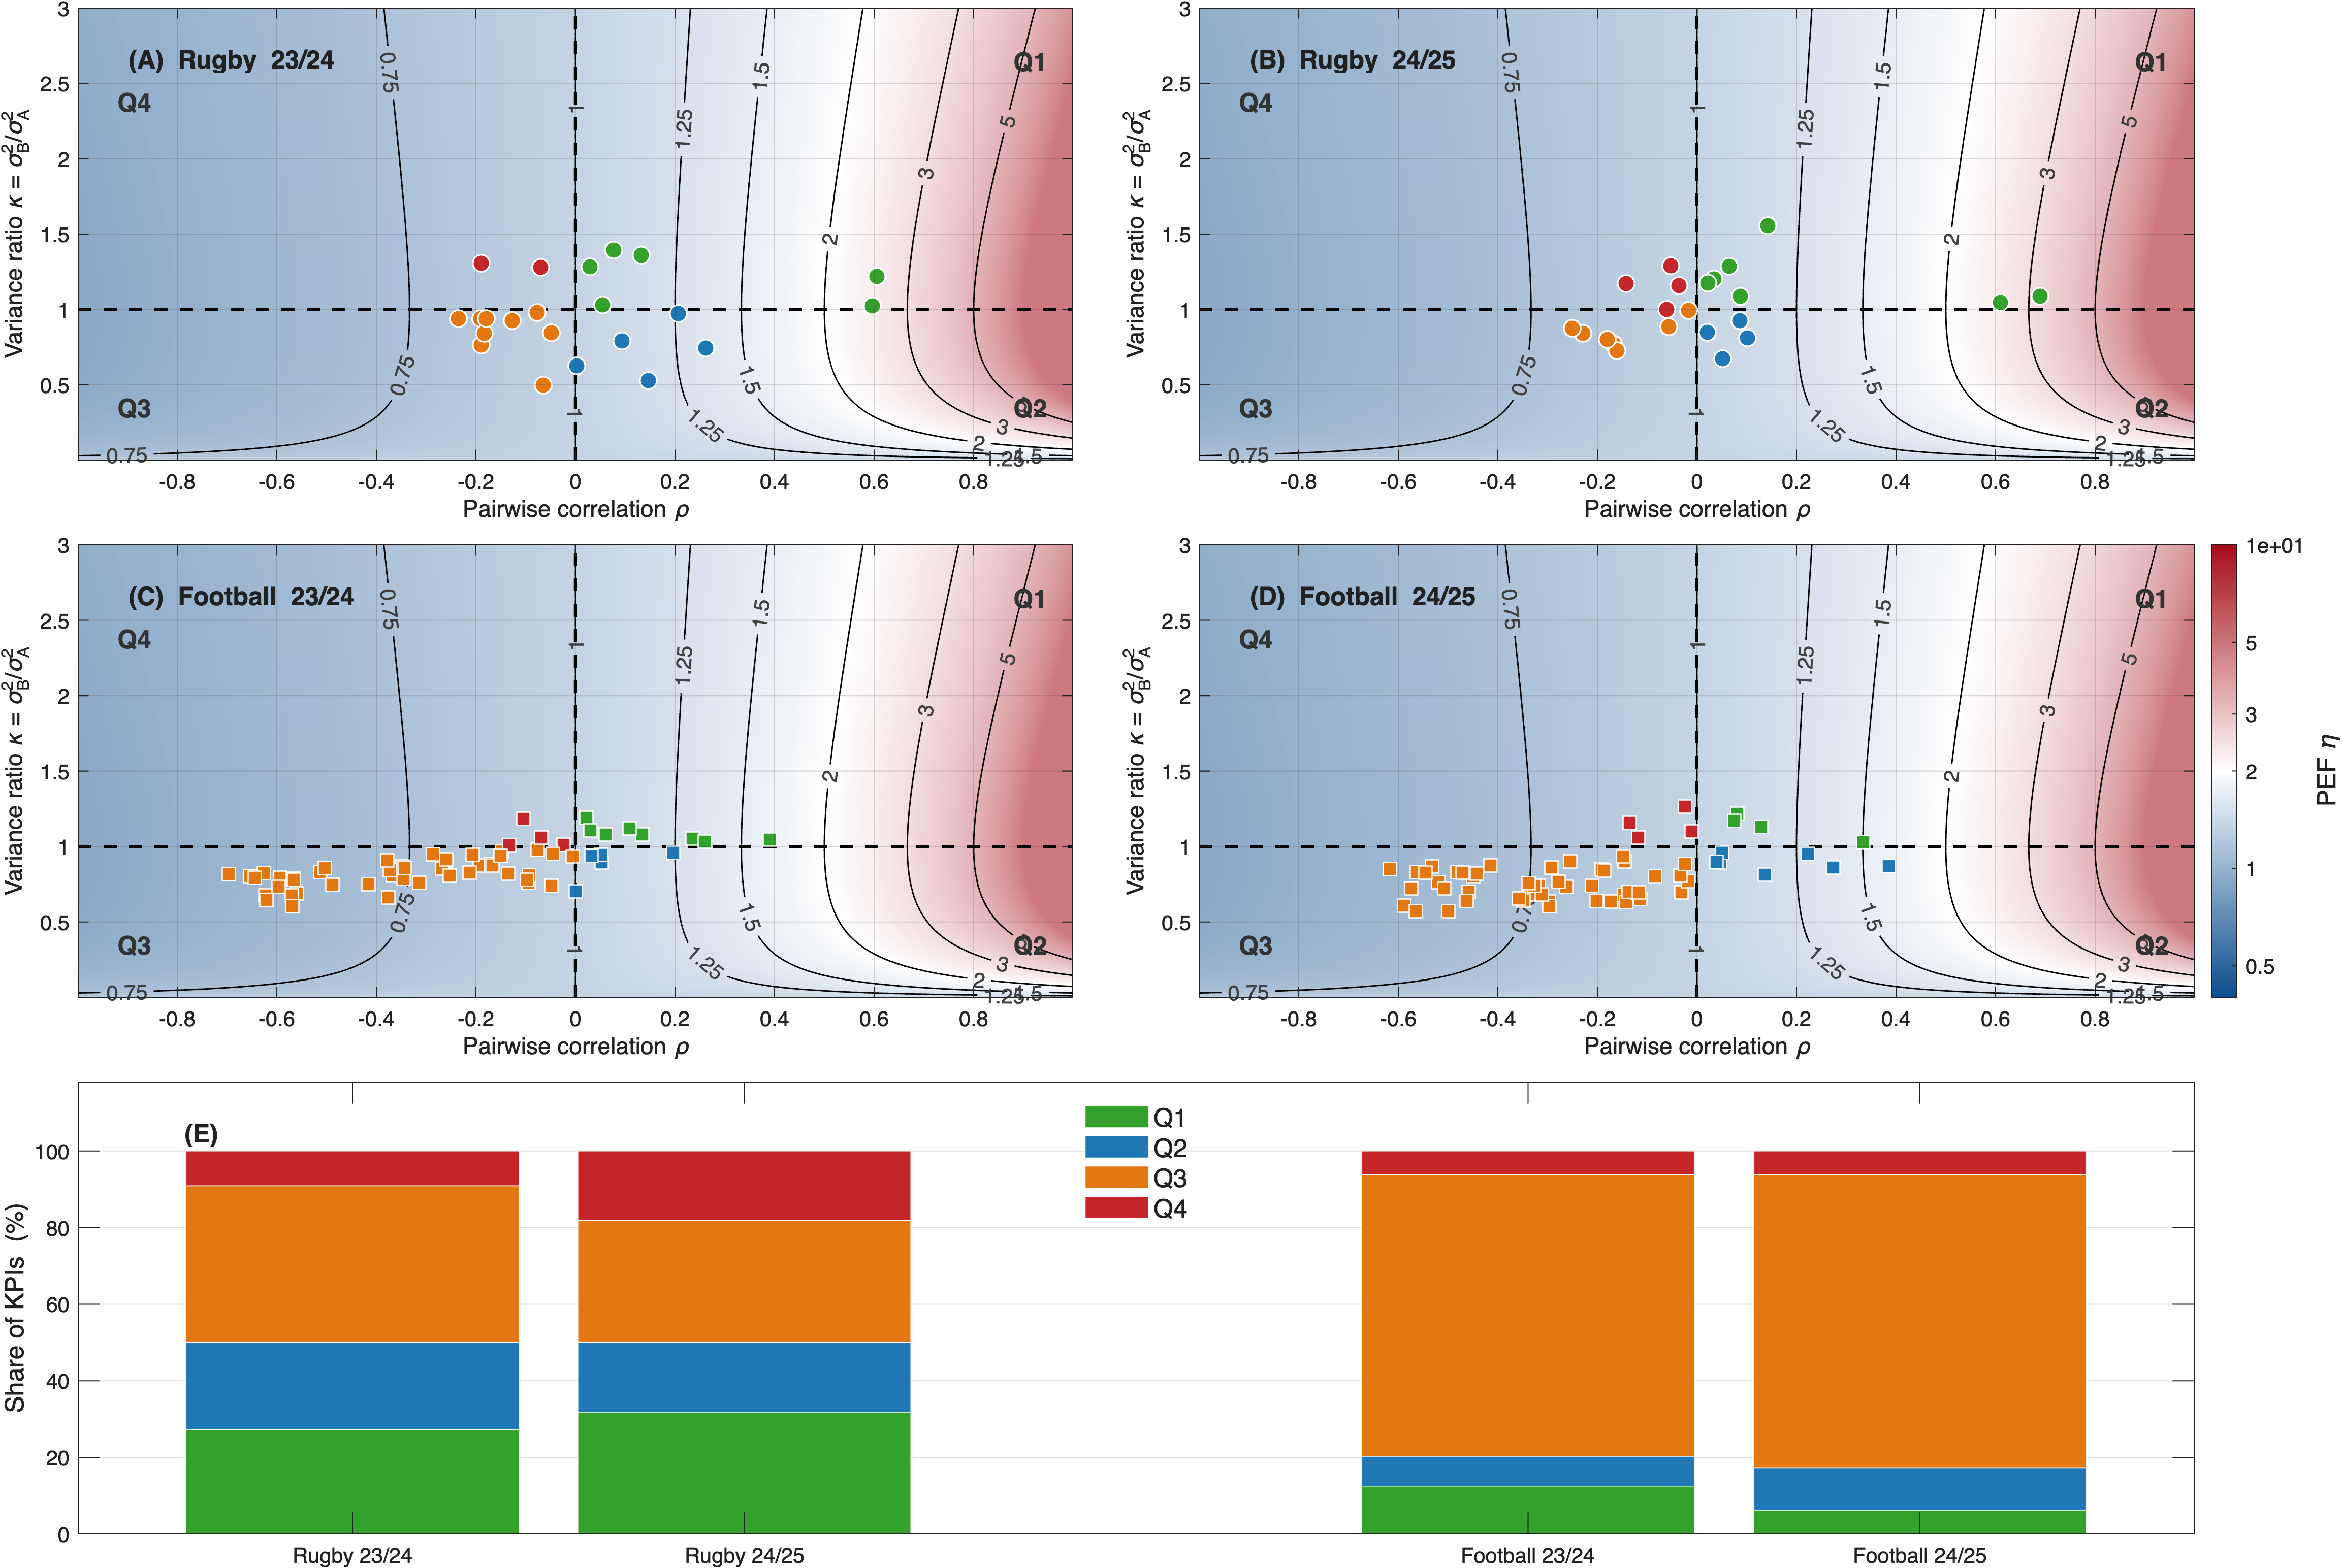
\includegraphics[width=\linewidth]{figures/Figure_S4_labelled_kpis.png}
  \caption{Sports KPI cloud on the $(\rho,\kappa)$ plane (rugby {URC}; football Championship;
    seasons 23/24--24/25). (A, B)~rugby; (C, D)~football. Markers are coloured by quadrant
    (Q1 green, Q2 blue, Q3 orange, Q4 red). (E)~share of KPIs in each quadrant, by season.
    Year-on-year identity is not traced.
    A minority of rugby KPIs cross a quadrant boundary between seasons.
    Football remains concentrated in Quadrant~3.
    The four exemplars are the rows of \cref{tab:exemplars}, not a separate panel.
    Class separation against $\Delta\mathrm{ML}$ is Supplementary~\cref{fig:si_ipred_vs_dml}.}
  \label{fig:pef_landscape}
\end{figure}



\printbibliography[title={References}]

%% Supplementary Information for the sports paper.
\clearpage
\setcounter{figure}{0}
\renewcommand{\thefigure}{S\arabic{figure}}
\setcounter{table}{0}
\renewcommand{\thetable}{S\arabic{table}}

\section*{Supplementary Information}

\noindent This supplement records data provenance, quality-control notes, and the classical derivations of alignment and the $1/(2n)$ cost used in the main text.
Further geometric identities appear in a companion manuscript \parencite{pefstatistics2026}.

\medskip
\noindent\begin{tabular}{@{}p{0.22\linewidth}p{0.34\linewidth}p{0.38\linewidth}@{}}
  \toprule
  \textbf{SI block} & \textbf{Main paper} & \textbf{Contents} \\
  \midrule
  \S1 Data note & Methods & Leagues, seasons, outcome coding \\
  \S2 Quality control & Methods & Bootstrap and leave-one-team-out notes \\
  \S3 Alignment and cost & Theory; Results & Classical derivations \\
  \bottomrule
\end{tabular}

\clearpage

% ---------------------------------------------------------------------------
\refstepcounter{sisection}
\section*{SI Section \thesisection: Data Note}
\label{sec:si_data}

\noindent Rugby KPIs are from the United Rugby Championship ($\PEFrugbyNgames$ matches; $\PEFrugbyNkpis$ KPIs).
Football KPIs are from the English Championship ($\PEFfootNgames$ matches; $\PEFfootNkpis$ KPIs).
Both windows pool seasons 23/24--24/25.
Home is $A$ and away is $B$.
The outcome is home win versus not; draws are coded as not a home win.
Neither league's match-level KPI file is redistributed (\cref{sec:data_availability}).

One row per KPI is written to \path{Alternative Pipeline/pef_numerics/results/E6_sports.csv}.
Second-moment estimates $(\hat\kappa,\hat\rho,\hat\eta)$ and quadrant labels are in \path{scripts/paper_pipeline/outputs/pef_landscape_2season.csv}.
The four pre-specified exemplars are listed in \path{scripts/paper_pipeline/outputs/confirmatory_exemplars.csv}.
Numeric macros in \path{scripts/paper_pipeline/outputs/sports_numbers.tex} are regenerated from those files without refitting.

\clearpage

% ---------------------------------------------------------------------------
\refstepcounter{sisection}
\section*{SI Section \thesisection: Quality Control}
\label{sec:si_qc}

\noindent Team-cluster bootstrap percentile intervals for $(\hat\kappa,\hat\rho,\hat\eta)$ use $B=1{,}000$ home-team resamples.
Away matches of a resampled club can remain in the bootstrap, because the cluster is the home team.
That design matches the landscape pipeline and is separate from leave-one-team-out log-loss (\cref{sec:ml_cv}).

Leave-one-team-out holds out one team $t$ at a time.
Test matches are those in which $t$ is home or away.
Training is the remaining matches, so the opponent's other fixtures stay in training.
Each match is scored once for each participating team that yields a valid fold, so a match typically contributes twice to the mean.
Uncertainty for per-KPI gaps and skill uses a team multinomial bootstrap: teams are redrawn with replacement, training weights are products of the two clubs' multiplicities, and out-of-bag matches form the test set.
Sport-level intervals for median gaps resample KPIs within sport.
The main text does not attach a $p$-value to one KPI's likelihood-ratio statistic.
Landmarks $\PEFLRaic$ and $\PEFLRlandmark$ on \cref{fig:e6_alignment} are references for feature choice and for a $\chi^2_1$ $5\%$ point, not discovery counts.

\clearpage

% ---------------------------------------------------------------------------
\refstepcounter{sisection}
\section*{SI Section \thesisection: Alignment and the Cost of a Redundant Coefficient}
\label{sec:si_alignment}

\noindent This section derives the two results used in the main text: the alignment condition behind the null $\beta_{\mathrm{A}}+\beta_{\mathrm{B}}=0$, and the finite-sample cost $1/(2n)$ of fitting the pair when the difference suffices.
Both are classical; we state them in the notation of this paper.

\subsection*{Alignment as a linear restriction}

Let $Y\in\{0,1\}$ indicate a home win, and let $A$ and $B$ be the home and away values of one KPI.
The pair model is
\begin{equation}
  \operatorname{logit}\Pr(Y=1\mid A,B)=\beta_{0}+\beta_{\mathrm{A}}A+\beta_{\mathrm{B}}B .
  \label{eq:si_pair}
\end{equation}
Writing $D=A-B$ and $S=A+B$, so that $A=(S+D)/2$ and $B=(S-D)/2$, the linear score becomes
\begin{equation}
  \beta_{\mathrm{A}}A+\beta_{\mathrm{B}}B
  =\tfrac12(\beta_{\mathrm{A}}-\beta_{\mathrm{B}})\,D
  +\tfrac12(\beta_{\mathrm{A}}+\beta_{\mathrm{B}})\,S .
  \label{eq:si_rotation}
\end{equation}
The difference model $\operatorname{logit}\Pr(Y=1\mid D)=\gamma_{0}+\gamma D$ is therefore the pair model with the single linear restriction $\beta_{\mathrm{A}}+\beta_{\mathrm{B}}=0$, with $\gamma=\beta_{\mathrm{A}}=-\beta_{\mathrm{B}}$.
When the restriction holds, $\Pr(Y=1\mid A,B)$ depends on $(A,B)$ only through $D$; within the model, $D$ is sufficient for the pair.
We call the KPI aligned in this case.
If the logistic model is misspecified, the same statements apply to the pseudo-true parameters that minimise expected log-loss \parencite{white1982}.

The restriction is invariant to centring and to rescaling $A$ and $B$ by a common factor, which is why both series are scaled by their pooled standard deviation.
Rescaling them by separate factors would change the null hypothesis.

Because the two models are nested and differ by one restriction, the likelihood-ratio statistic $\Lambda=2(\ell_{(\mathrm{A},\mathrm{B})}-\ell_{D})$ is asymptotically $\chi^{2}_{1}$ under the null for independent observations \parencite{wilks1938}.
Under local misalignment it is approximately noncentral $\chi^{2}_{1}$ with noncentrality $\lambda$, so that $\mathbb{E}[\Lambda]\approx 1+\lambda$.
Team recurrence makes matches dependent, so the $\chi^{2}_{1}$ reference is a landmark here rather than a calibrated null.

\subsection*{Expected excess test log-loss of a fitted model}

Let $\ell(\theta;x,y)$ be the log-likelihood of one observation under a regular parametric model with $k$ free parameters, and let $R(\theta)=-\mathbb{E}\,\ell(\theta;X,Y)$ be its expected log-loss on a new observation.
Let $\theta^{*}$ minimise $R$, and let $\hat\theta$ be the maximum-likelihood estimate from $n$ independent training observations.
A second-order expansion of $R$ about $\theta^{*}$ gives
\begin{equation}
  R(\hat\theta)\approx R(\theta^{*})
  +\tfrac12(\hat\theta-\theta^{*})^{\top}J\,(\hat\theta-\theta^{*}),
  \qquad J=\mathbb{E}\bigl[-\nabla^{2}\ell(\theta^{*};X,Y)\bigr].
\end{equation}
Since $\sqrt{n}(\hat\theta-\theta^{*})\to\mathcal{N}(0,J^{-1}KJ^{-1})$ with $K=\mathbb{E}\bigl[\nabla\ell\,\nabla\ell^{\top}\bigr]$ \parencite{white1982},
\begin{equation}
  \mathbb{E}\bigl[R(\hat\theta)\bigr]-R(\theta^{*})
  \approx\frac{\operatorname{tr}(J^{-1}K)}{2n}.
  \label{eq:si_excess}
\end{equation}
When the model is correctly specified, $K=J$ and the excess is $k/(2n)$.
This is the per-parameter penalty underlying Akaike's information criterion \parencite{akaike1973}; \cref{eq:si_excess} is the general form behind Takeuchi's criterion \parencite{konishi2008}.
No distributional assumption on the features is required beyond regularity.

\subsection*{The cost of fitting the pair when the difference suffices}

Suppose the KPI is aligned.
The pseudo-true pair parameter then satisfies the restriction, so the pair model (three parameters) and the difference model (two parameters) attain the same population risk $R(\theta^{*})$.
Applying \cref{eq:si_excess} to each model with correct specification,
\begin{equation}
  \mathbb{E}\bigl[\mathrm{LL}(D)-\mathrm{LL}(A,B)\bigr]
  \approx\frac{2}{2n}-\frac{3}{2n}=-\frac{1}{2n}.
  \label{eq:si_cost}
\end{equation}
Fitting the pair spends one redundant coefficient, and the difference is expected to have lower test log-loss by about $1/(2n)$ nats per match.
Under cross-validation, $n$ is the size of each training set, not the full sample.

If the KPI is not aligned, let $\Delta^{*}>0$ be the population log-loss lost by imposing the restriction.
The expected gap becomes
\begin{equation}
  \mathbb{E}\bigl[\mathrm{LL}(D)-\mathrm{LL}(A,B)\bigr]
  \approx\Delta^{*}-\frac{1}{2n},
  \label{eq:si_crossover}
\end{equation}
so the difference is still expected to predict better whenever the misalignment costs less than the redundant coefficient.
Under local alternatives the noncentrality of $\Lambda$ is $\lambda\approx2n\Delta^{*}$, so the crossover $\Delta^{*}=1/(2n)$ corresponds to $\lambda=1$, that is to $\mathbb{E}[\Lambda]\approx 2$.
This is Akaike's threshold for choosing between nested models that differ by one parameter, and it matches the asymptotic equivalence between Akaike's criterion and cross-validation \parencite{stone1977}.
For out-of-sample feature choice, $\Lambda=2$ is therefore the natural landmark; the $\chi^{2}_{1}$ $5\%$ point $3.84$ answers a different question (rejecting exact alignment).

\subsection*{Scope}

The expansions are first-order in $1/n$ and assume independent observations and a regular model.
Team recurrence and leave-one-team-out folds make matches dependent and folds unequal, so \cref{eq:si_cost,eq:si_crossover} are approximations for these leagues rather than exact predictions.
Under misspecification, $1/(2n)$ in \cref{eq:si_cost} is replaced by the difference in the two models' values of $\operatorname{tr}(J^{-1}K)/(2n)$.


\end{document}
